\documentclass{beamer}
\usetheme{Madrid}

\AtBeginSection[]{
  \begin{frame}
  \vfill
  \centering
  \begin{beamercolorbox}[sep=8pt,center,shadow=true,rounded=true]{title}
    \usebeamerfont{title}\insertsectionhead\par%
  \end{beamercolorbox}
  \vfill
  \end{frame}
}


\usepackage{amsmath}
\usepackage{amssymb}
\usepackage{amsthm}
\usepackage{multicol}
\theoremstyle{remark}
\newtheorem{remark}{Remark}
\usepackage{mathtools}
\usepackage[]{graphicx}
\usepackage{libertinus}
\usepackage{caption}
\usepackage{subcaption}
\usepackage[backend=biber]{biblatex}
\addbibresource{bibliography.bib}

\newcommand{\gammabf}{\boldsymbol{\gamma}}
\newcommand{\const}{\, \text{const.}}
\newcommand{\xbf}{\mathbf{x}}
\newcommand{\ybf}{\mathbf{y}}
\newcommand{\intd}{\, \text{d}}
\newcommand{\norm}[1]{\lvert \lvert #1 \rvert \rvert}
\newcommand{\inner}[1]{\langle \langle #1 \rangle \rangle}

\DeclareMathOperator{\grad}{grad}

\setlength{\columnseprule}{1pt}


\title{Untangling Knots Through Curve Repulsion}
\titlegraphic{
\includegraphics[height=2cm]{oxfordlogo.eps}}
\author{Joo-Hyun Paul Kim}

\begin{document}

% Title Page
\begin{frame}
    \titlepage
\end{frame}

\begin{frame}
    \frametitle{What the curious folks ponder about}
    \tableofcontents
\end{frame}

\section{Introduction}
\begin{frame}
    \frametitle{A Cool Knot}
    \begin{figure}[h]
        \centering
        \includegraphics[scale=0.25]{knot}
        \caption{Imagine your earphones getting tangled like this\ldots}
    \end{figure}
\end{frame}


\begin{frame}
    \frametitle{Aim}
    \begin{itemize}
        \item<1-> Finding a ``homotopy'' from a knot to an unknot.
            \begin{figure}[h]
                \centering
                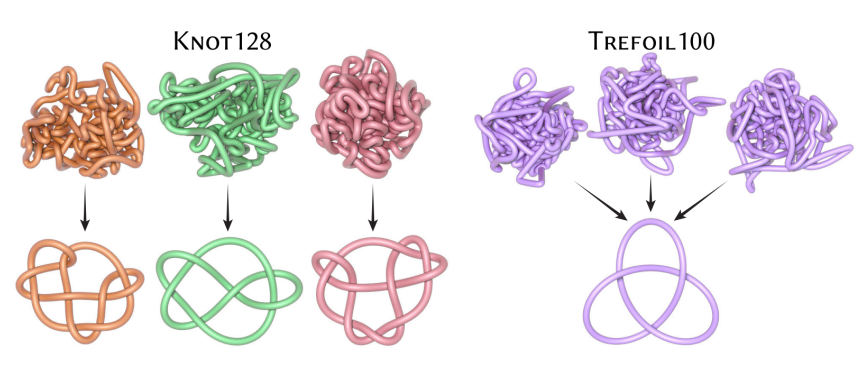
\includegraphics[scale=0.2]{knotsolving}
                \caption{Unknots of test knots.\cite{YSC2021}}
            \end{figure}
        \item<2-> ``Avoiding self-intersection''
    \end{itemize}
\end{frame}

\begin{frame}
    \frametitle{General Strategy}
    \begin{enumerate}
        \item<1-> Define curve energy; penalizing the closeness of points on a curve.
            \begin{itemize}
                \item Extreme-closeness of points on curve is a natural characteristic of a tangled curve.
            \end{itemize}
        \item<2-> Attempt to decrease the curve energy by continuously deforming the curve.
            \begin{itemize}
                \item We evolve the curve according to the gradient flow equation.
                \item There is a freedom in choosing the ``gradient'' here.
            \end{itemize}
        \item<3-> We expect the stationary state to be the ``unknot''
            \begin{itemize}
                \item Or at least a simpler state\ldots
            \end{itemize}
    \end{enumerate}

\end{frame}

\section{Tangent-Point Energy}
\begin{frame}
    \frametitle{Defining Curve Energy}
    \onslide<1->{
        Given an (arc-length parameterised) curve $\gammabf:M \rightarrow \mathbb{R}^3$, we wish to assign energy of the form:
        \begin{equation}
            \mathcal{E} \left( \gammabf \right) \coloneqq \iint_{M^2} k \left( \gammabf_x, \gammabf_y \right) \intd \gamma_x \intd \gamma_y
        \end{equation}
        such that
        \begin{itemize}
            \item $\mathcal{E}$ is very high when two non-neighbouring points are very close.
        \end{itemize}
    }
    \onslide<2>{
        A na\"ive choice is $k \left( \gammabf_x, \gammabf_y \right) \coloneqq \frac{1}{\norm{\gammabf_x - \gammabf_y}}$
    }
\end{frame}

\begin{frame}
    \frametitle{Pitfall of the ``Simple Energy''}
        \begin{equation*}
            \mathcal{E} \left( \gammabf \right) \coloneqq \iint_{M^2} \frac{1}{\norm{\gammabf_x - \gammabf_y}} \intd \gamma_x \intd \gamma_y
        \end{equation*}
        \begin{figure}[h]
            \centering
            \begin{subfigure}[b]{0.45\textwidth}
                \centering
                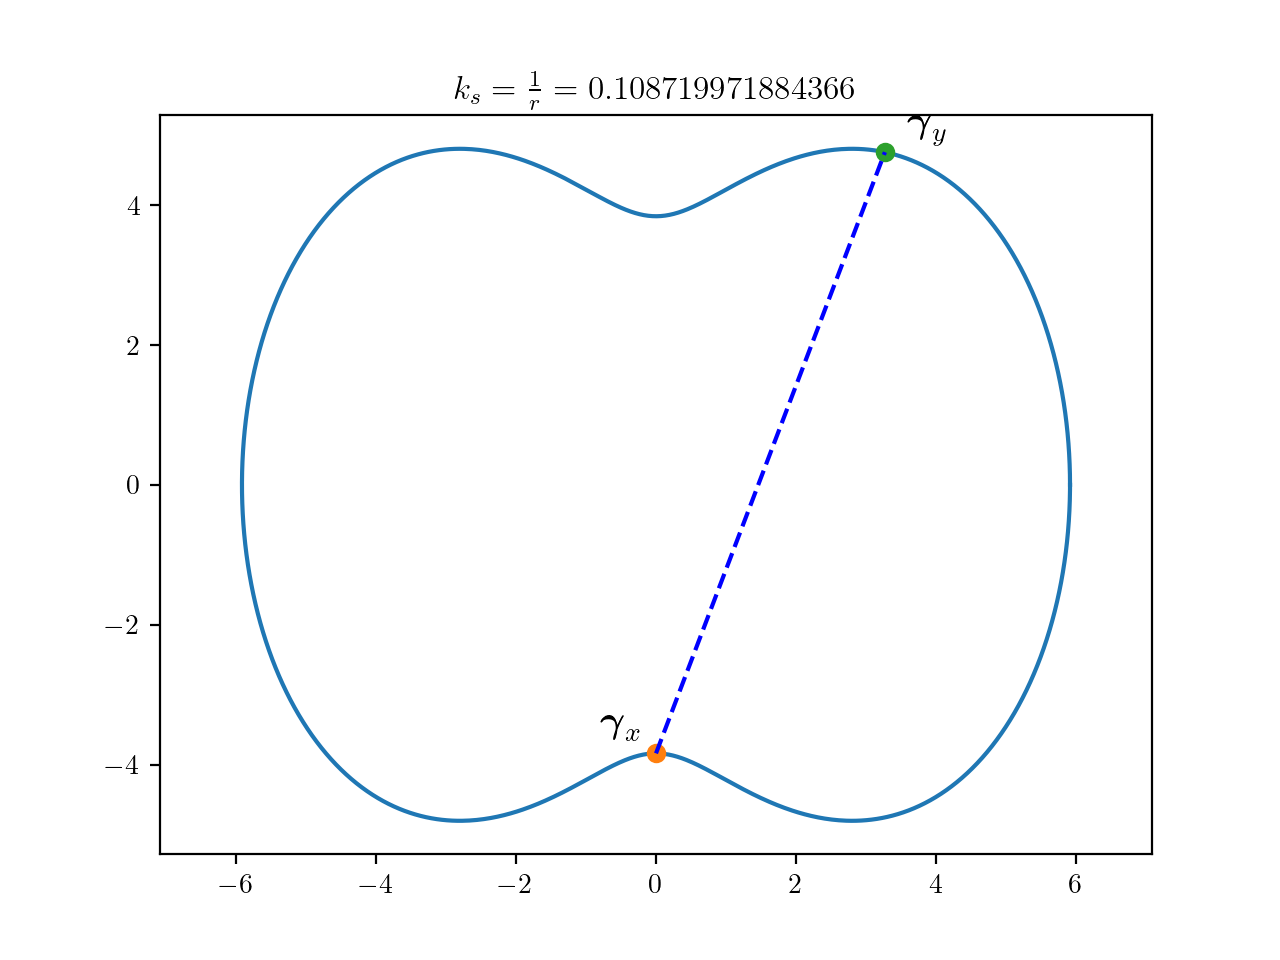
\includegraphics[width=\textwidth]{simple-0}
            \end{subfigure}
            \begin{subfigure}[b]{0.45\textwidth}
                \centering
                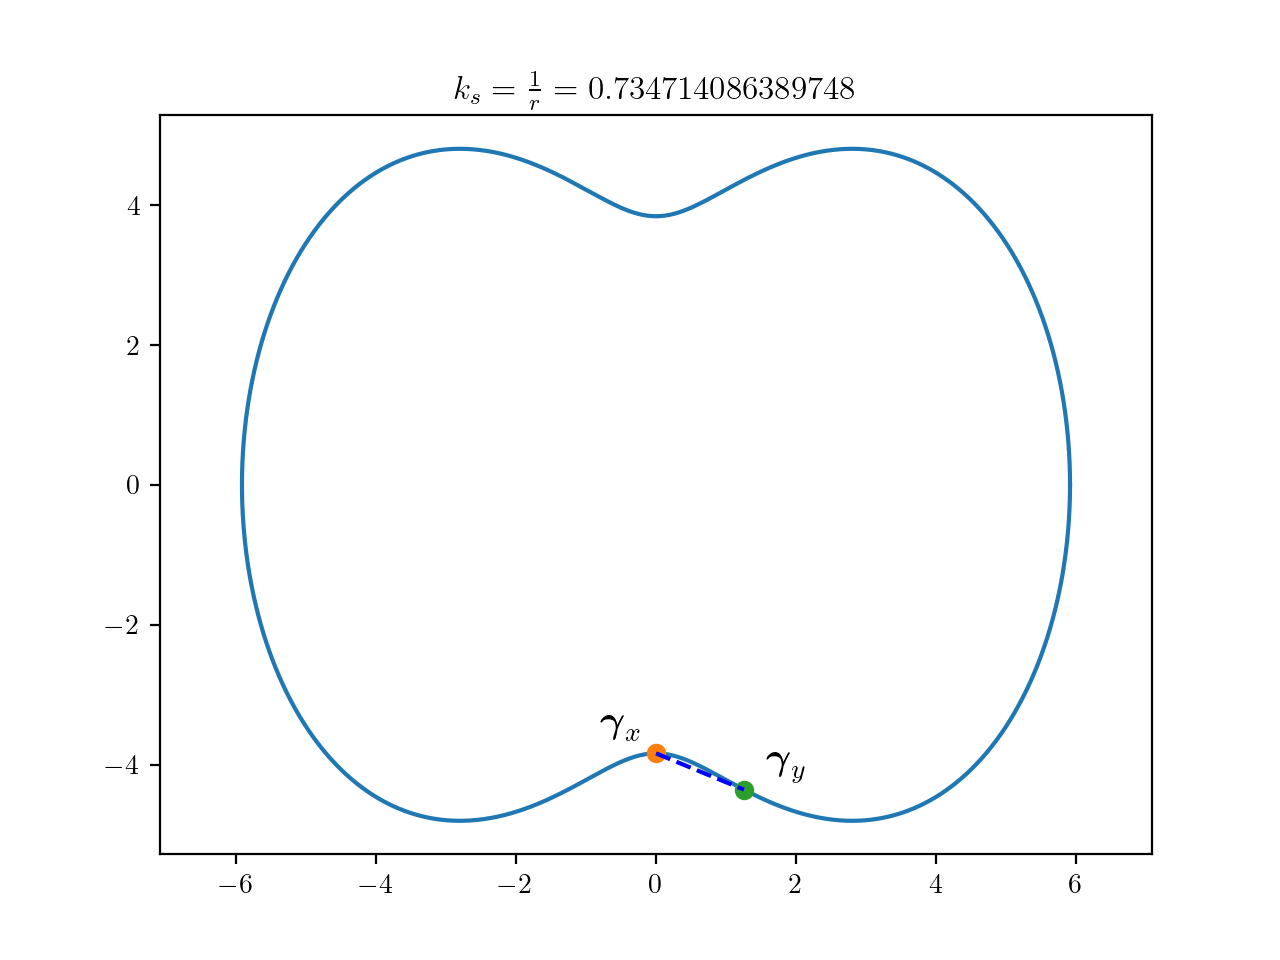
\includegraphics[width=\textwidth]{simple-1}
            \end{subfigure}
        \end{figure}
\end{frame}

\begin{frame}
    \frametitle{Pitfall of the ``Simple Energy''}
        \begin{equation*}
            \mathcal{E} \left( \gammabf \right) \coloneqq \iint_{M^2} \frac{1}{\norm{\gammabf_x - \gammabf_y}} \intd \gamma_x \intd \gamma_y
        \end{equation*}
        \begin{figure}[h]
            \centering
            \begin{subfigure}[b]{0.45\textwidth}
                \centering
                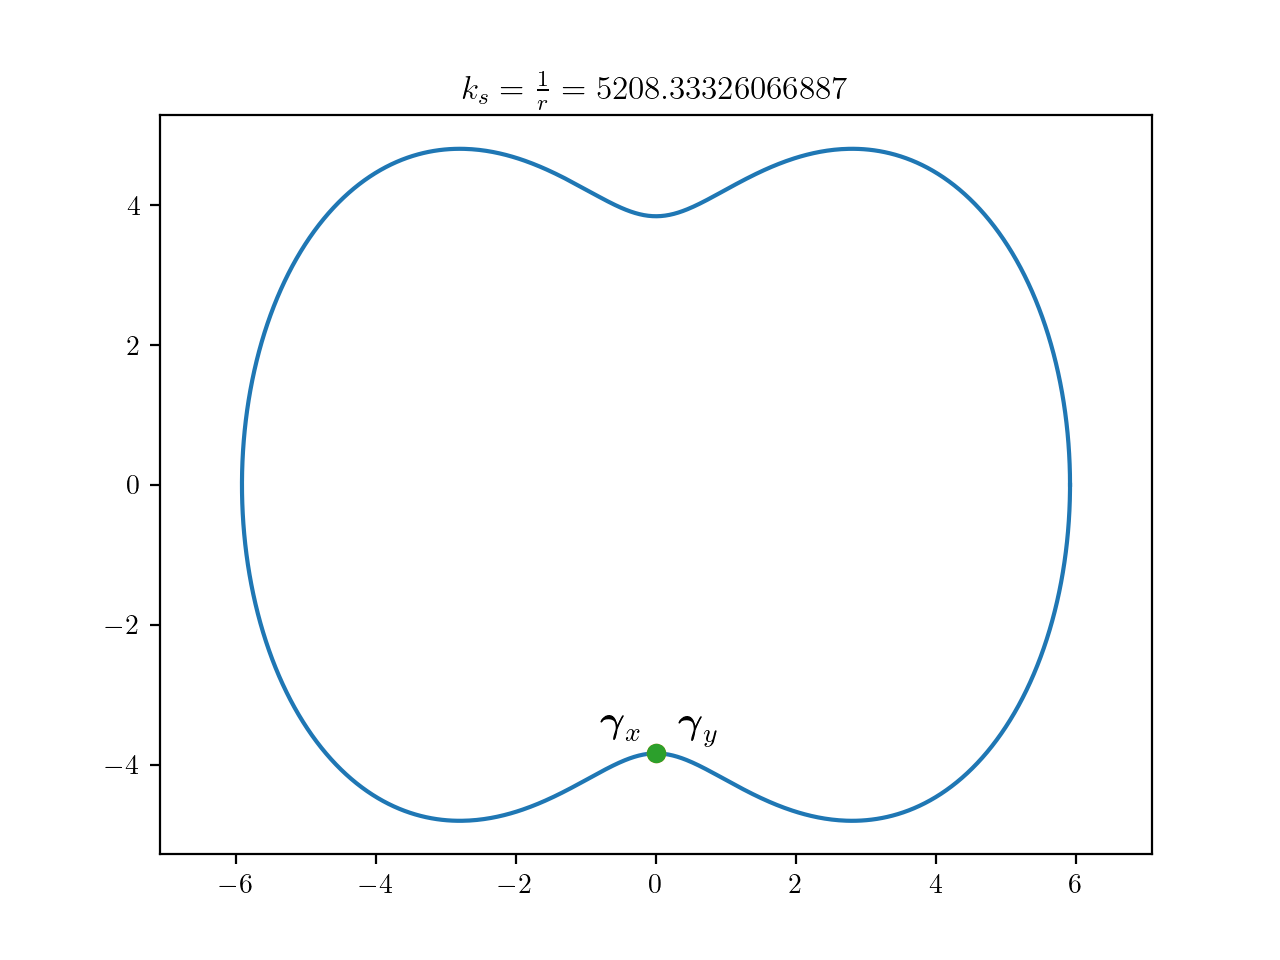
\includegraphics[width=\textwidth]{simple-2}
            \end{subfigure}
            \begin{subfigure}[b]{0.45\textwidth}
                \centering
                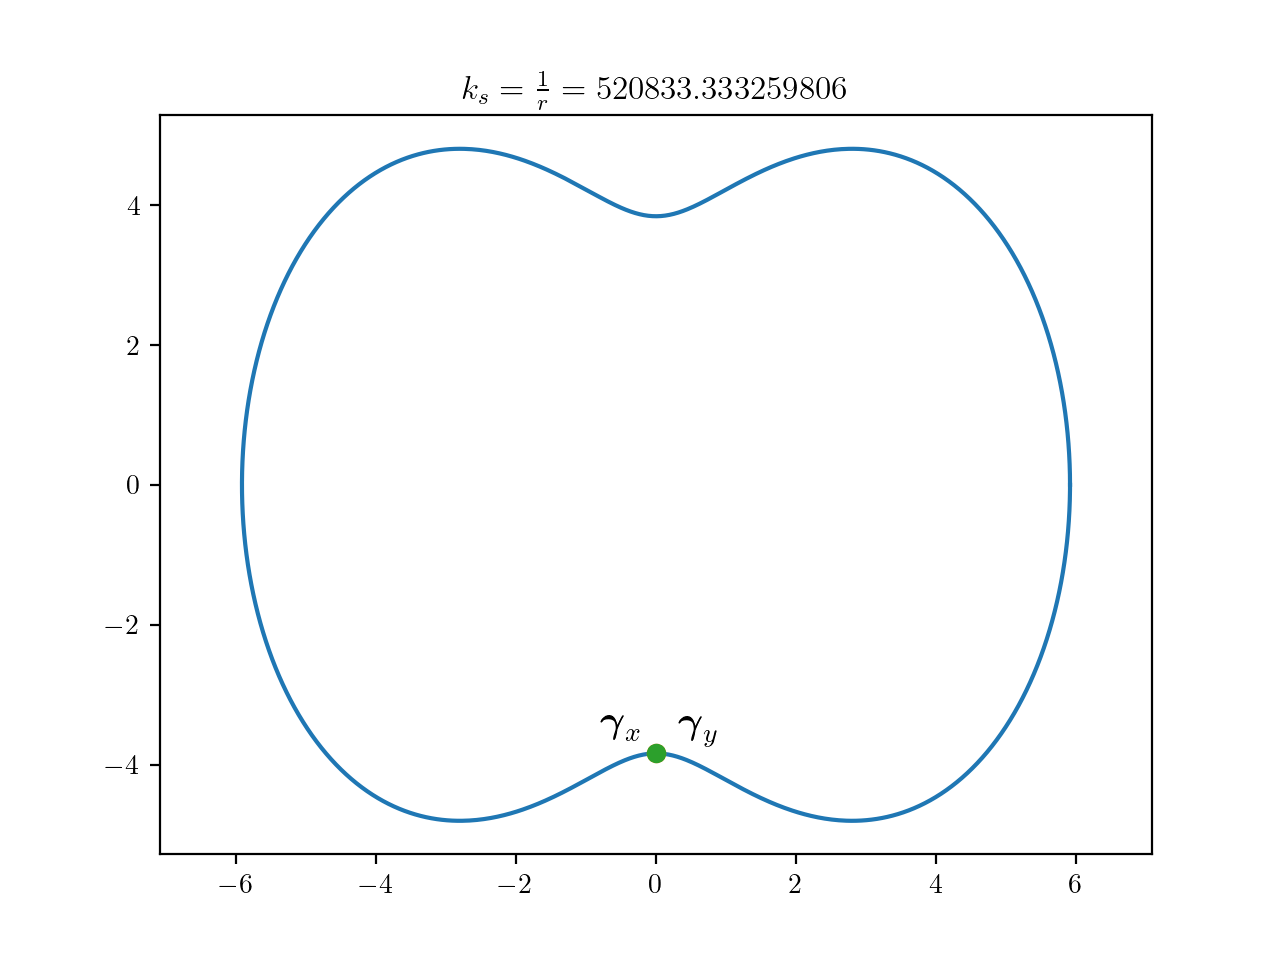
\includegraphics[width=\textwidth]{simple-3}
            \end{subfigure}
        \end{figure}
        \onslide<2->{
            This energy is not well-defined for a lot of curves!
        }
\end{frame}

\begin{frame}
    \frametitle{Buck-Orloff Tangent-Point Energy}
    \begin{itemize}
        \item From the simple energy, need a way to suppress the infinite contribution of the ``singularity''.
    \end{itemize}
    \begin{definition}[Buck-Orloff Tangent-Point Energy]<2->
        For a smooth curve $\gammabf$, define
        \begin{equation*}
            \mathcal{E} \left( \gammabf \right) \coloneqq \iint_{M^2} k_{4}^2 \left( \gammabf_x, \gammabf_y, \mathbf{T}_x \right) \intd \gamma_x \intd \gamma_y
        \end{equation*}
        where $\mathbf{T}_x$ is the unit tangent vector at $\gammabf_x$,
        with the kernel defined as
        \begin{equation*}
            k_4^2 \left( \mathbf{p}, \mathbf{q}, \mathbf{T} \right) \coloneqq \frac{\norm{\mathbf{T} \wedge \left( \mathbf{p} - \mathbf{q} \right)}^{2}}{\norm{\mathbf{p} - \mathbf{q}}^{4}}
        \end{equation*}
        as \textbf{Buck-Orloff Tangent-Point Energy}.\cite{BO1995}
    \end{definition}
\end{frame}

\begin{frame}
    \frametitle{Intuition}
    What is the intuition behind the kernel $k_4^2 \left( \mathbf{p}, \mathbf{q}, \mathbf{T} \right) \coloneqq \frac{\norm{\mathbf{T} \wedge \left( \mathbf{p} - \mathbf{q} \right)}^{2}}{\norm{\mathbf{p} - \mathbf{q}}^{4}}$?

    \onslide<2->
    {
        \begin{figure}[h]
            \centering
            \begin{subfigure}[b]{0.48\textwidth}
                \centering
                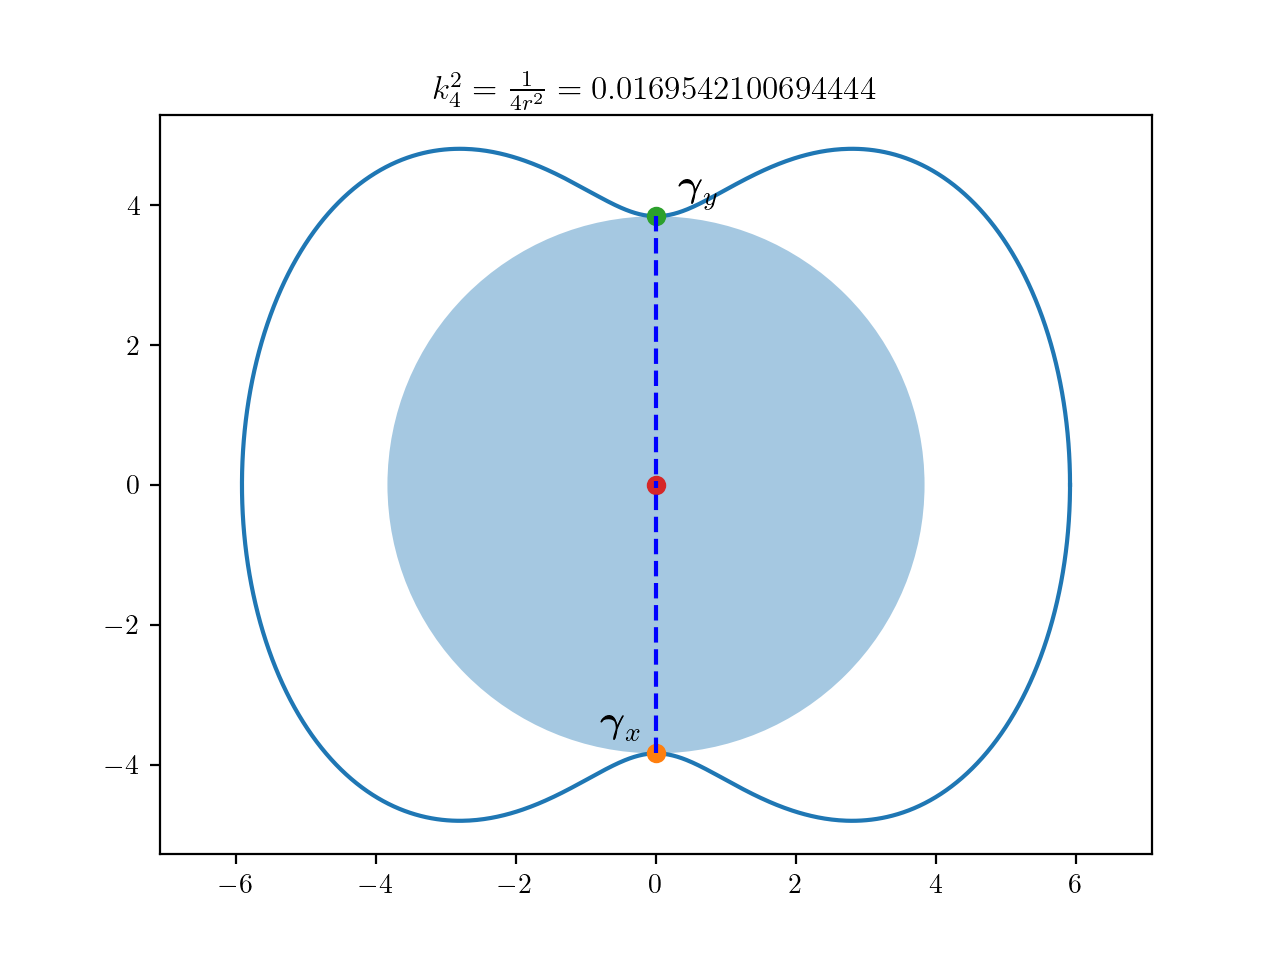
\includegraphics[width=\textwidth]{straight}
            \end{subfigure}
            \begin{subfigure}[b]{0.48\textwidth}
                \centering
                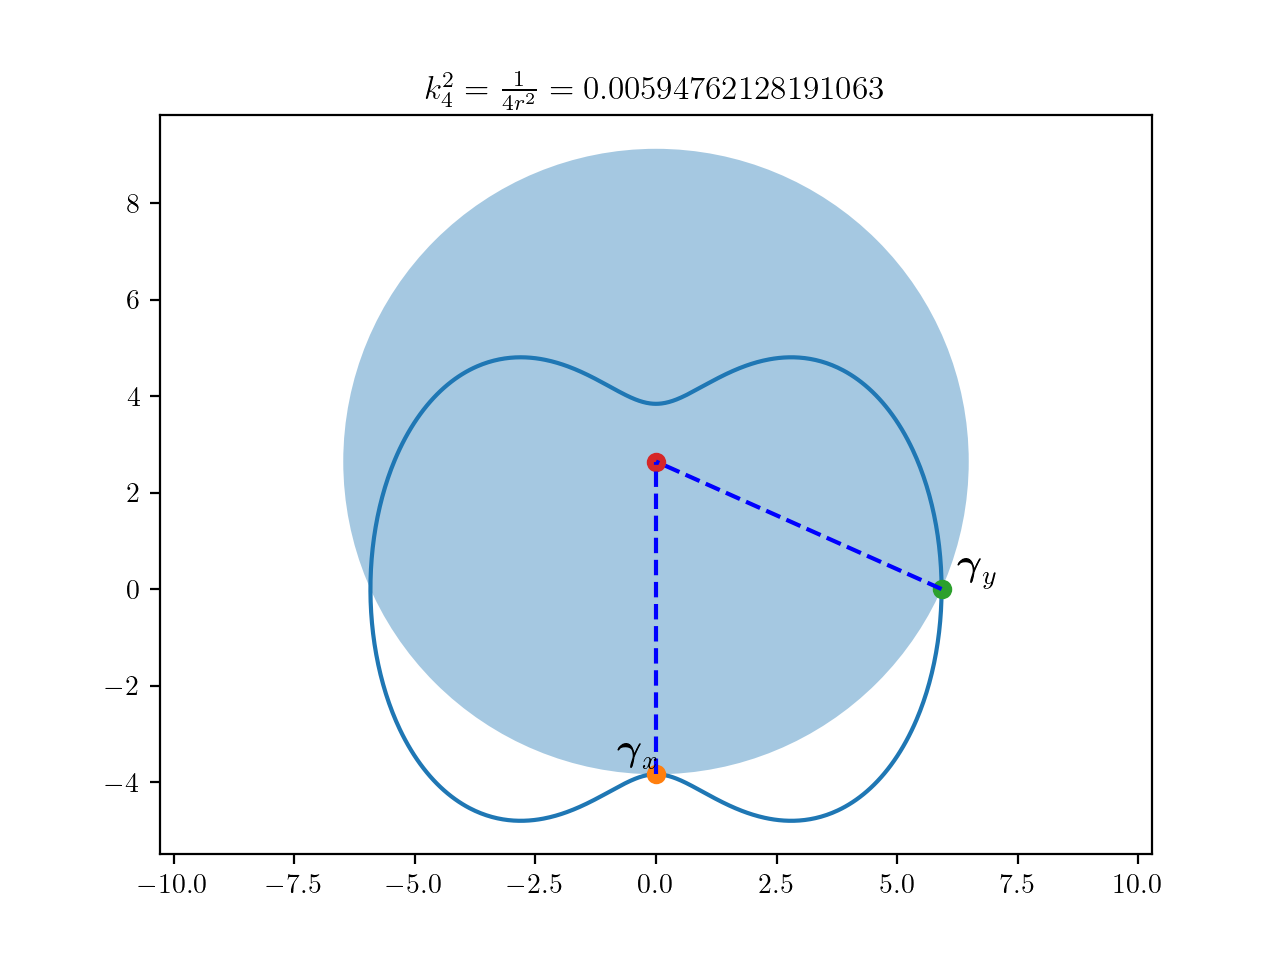
\includegraphics[width=\textwidth]{0}
            \end{subfigure}
        \end{figure}
    }

    \begin{remark}<3->
        Note that closer does not necessarily mean the kernel is larger.
    \end{remark}
\end{frame}

\begin{frame}
    \frametitle{Intuition}
    \begin{figure}[h]
        \centering
        \includegraphics[scale=0.5]{perturbed}
        \caption{When two points are very close, the kernel converges to the curvature of the curve.}
    \end{figure}
\end{frame}

\begin{frame}
    \frametitle{Example: Buck-Orloff Tangent-Point Energy of a Circle}
    \begin{example}
        Suppose we wish to compute the Buck-Orloff tangent-point energy of a unit circle.
        \onslide<2->
        {
            Parameterise unit circle as:
            \begin{multicols}{2}
            \begin{equation*}
                \gammabf (t) = \left( \cos{t}, \sin{t}, 0 \right)
            \end{equation*}
            \columnbreak
            \begin{figure}[h]
                \centering
                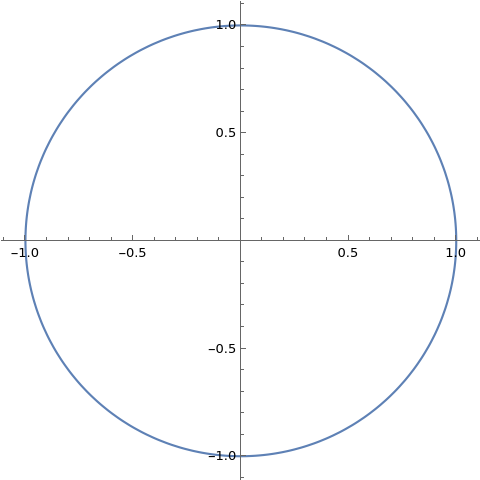
\includegraphics[scale=0.2]{unitcircle}
            \end{figure}
            \end{multicols}
        }
        \onslide<3->
        {
            Then write:
            \begin{equation*}
                \begin{cases}
                    \gammabf_x \left( \theta \right) = \left( \cos{\theta}, \sin{\theta}, 0 \right) \\
                    \gammabf_y \left( \phi \right) = \left( \cos{\phi}, \sin{\phi}, 0 \right) \\
                    \mathbf{T}_x \left( \theta \right) = \left( -\sin{\theta}, \cos{\theta}, 0 \right)
                \end{cases}
            \end{equation*}
        }
    \end{example}
\end{frame}

\begin{frame}
    \begin{example}[Cont.]
            \begin{equation*}
                \begin{cases}
                    \gammabf_x \left( \theta \right) = \left( \cos{\theta}, \sin{\theta}, 0 \right) \\
                    \gammabf_y \left( \phi \right) = \left( \cos{\phi}, \sin{\phi}, 0 \right) \\
                    \mathbf{T}_x \left( \theta \right) = \left( -\sin{\theta}, \cos{\theta}, 0 \right)
                \end{cases}
            \end{equation*}
            Substituting to Buck-Orloff Tangent-Point energy formula:
        \begin{equation*}
            \mathcal{E} \left( \gammabf \right) \coloneqq \iint_{M^2} \frac{\norm{\mathbf{T}_x \wedge \left( \gammabf_x - \gammabf_y \right)}^{2}}{\norm{\gammabf_x - \gammabf_y}^{4}} \intd \gamma_x \intd \gamma_y
        \end{equation*}
        \onslide<2->
        {
            Using a few identities:
            \begin{align*}
                \mathcal{E} \left( \gammabf \right) &= \int_{\theta=0}^{2 \pi} \int_{\phi=0}^{2 \pi}
                \frac{\norm{\mathbf{T}_x}^2 \norm{\gammabf_x - \gammabf_y}^2 - \left( \mathbf{T}_x \cdot \left( \gammabf_x -\gammabf_y \right) \right)^2}{\norm{\gammabf_x - \gammabf_y}^4} \intd \theta \intd \phi
            \end{align*}
        }
    \end{example}
\end{frame}

\begin{frame}
    \begin{example}[Cont.]
        \begin{align}
            \mathcal{E} \left( \gammabf \right) &= \int_{\theta=0}^{2 \pi} \int_{\phi=0}^{2 \pi}
            \frac{\norm{\mathbf{T}_x}^2 \norm{\gammabf_x - \gammabf_y}^2 - \left( \mathbf{T}_x \cdot \left( \gammabf_x -\gammabf_y \right) \right)^2}{\norm{\gammabf_x - \gammabf_y}^4} \intd \theta \intd \phi \\
            &= \int_{\theta=0}^{2 \pi} \int_{\phi=0}^{2 \pi}
            \frac{\sin^2 \frac{\theta - \phi}{2}}{\left( -1 + \cos \left( \theta - \phi \right) \right)^2} \intd \theta \intd \phi \\
            &= \int_{\theta=0}^{2 \pi} \int_{\phi=0}^{2 \pi}
            \frac{\sin^2 \frac{\theta - \phi}{2}}{\sin^4 \frac{\theta - \phi}{2}} \intd \theta \intd \phi
            \label{equ: 1 over r squared order}
            \\
            &= \pi^2
        \end{align}
    \end{example}
    \begin{remark}<2->
        Note that (\ref{equ: 1 over r squared order}) suggests the order at ``singularity'' is inverse-square.
    \end{remark}
\end{frame}

\begin{frame}
    \frametitle{General Tangent-Point Energy}
    A more general form of tangent-point energy comes from Yu, Schumacher, and Crane \cite{YSC2021}:
    \begin{definition}[Generalised Tangent-Point Energy]
        \begin{equation*}
            \mathcal{E}_{\beta}^{\alpha} \left( \gammabf \right) \coloneqq
            \iint_{M^2} \frac{\norm{\mathbf{T}_x \wedge \left( \gammabf_x - \gammabf_y \right)}^{\alpha}}{\norm{\gammabf_x - \gammabf_y}^{\beta}}
            \intd \gamma_x \intd \gamma_y
        \end{equation*}
        where $\alpha > 1$ and $\beta \in \left[ \alpha+2, 2\alpha+1 \right)$
    \end{definition}
    \begin{remark}
        When $\alpha = 2$ and $\beta = 4$, we are back to Buck-Orloff.
    \end{remark}
\end{frame}

\section{Gradient Flow}
\begin{frame}
    \frametitle{Motivating Gradient Flow}
    A simple method of minimising a (differentiable) function $f:\mathbb{R}^n \rightarrow \mathbb{R}$ is the steepest descent \cite{doi:10.1137/1.9781611974997.ch8}
    \begin{equation}
        \xbf^{k+1} = \xbf^k - \alpha_k \nabla f \left( \xbf^k \right)
    \end{equation}
    where $\alpha^k > 0$.
    \begin{figure}[h]
        \centering
        \includegraphics[scale=0.2]{sdm}
        \caption{Steepest Descent}
    \end{figure}
    \onslide<2->
    {
        For motivation, take $\alpha^k = \alpha \equiv \const$
    }
\end{frame}

\begin{frame}
    \begin{equation*}
        \xbf^{k+1} = \xbf^k - \alpha_k \nabla f \left( \xbf^k \right)
    \end{equation*}
    In the case of functional $\mathcal{E}: X \rightarrow \mathbb{R}$, analogously write steepest descent step:
    \begin{equation*}
        f^{k+1} = f^k - \alpha \grad_X f
    \end{equation*}
    \onslide<2->
    {
        Rearranging and dividing by $\Delta t$
        \begin{equation*}
            \frac{1}{\Delta t} \left( f^{k+1} - f^k \right) = -\alpha \grad_X f
        \end{equation*}
    }
    \onslide<3->
    {
        Take limit as $\Delta t \rightarrow 0$, then scale time variable to nondimensionalise to get the gradient flow equation.
        \begin{definition}[Gradient Flow Equation]
            \begin{equation*}
                \frac{\partial f}{\partial t} = - \grad_X f
            \end{equation*}
        \end{definition}
        But what is $\grad_X f$?
    }
\end{frame}

\begin{frame}
    \frametitle{Gradient in Space of Function?}

    \begin{multicols}{2}
        (Gradient of Function)

        $\nabla f\left( \xbf \right)$ is such that
        for all $\ybf \in \mathbb{R}^n$
        \begin{equation*}
            \left.\nabla f \left( \xbf \right) \cdot \ybf = \frac{\partial}{\partial \epsilon} f \left( \xbf + \epsilon \ybf \right)\right|_{\epsilon = 0}
        \end{equation*}
        \columnbreak

        (Gradient of Functional)

        $\grad_X E \left( f \right)$ is such that
        for all $g \in X$,
        \begin{equation*}
            \left.\inner{\grad_X E, g}_X = \frac{\partial}{\partial \epsilon} E \left( f + \epsilon g \right)\right|_{\epsilon = 0}
        \end{equation*}
    \end{multicols}
    
\end{frame}

\begin{frame}
    \frametitle{Bibliography}
    \printbibliography
\end{frame}

\end{document}
